%!TEX root = ../Thesis.tex

%%%%%%%%%%%%%%%%%%%%%%%%%%%%%%%%%%%%%%%%%%%%%%%%%%%%%%%%%%%%%%%%%%%%%%%%
\chapter{Introduction}
%%%%%%%%%%%%%%%%%%%%%%%%%%%%%%%%%%%%%%%%%%%%%%%%%%%%%%%%%%%%%%%%%%%%%%%%

\begin{figure}[t]
  \centering
  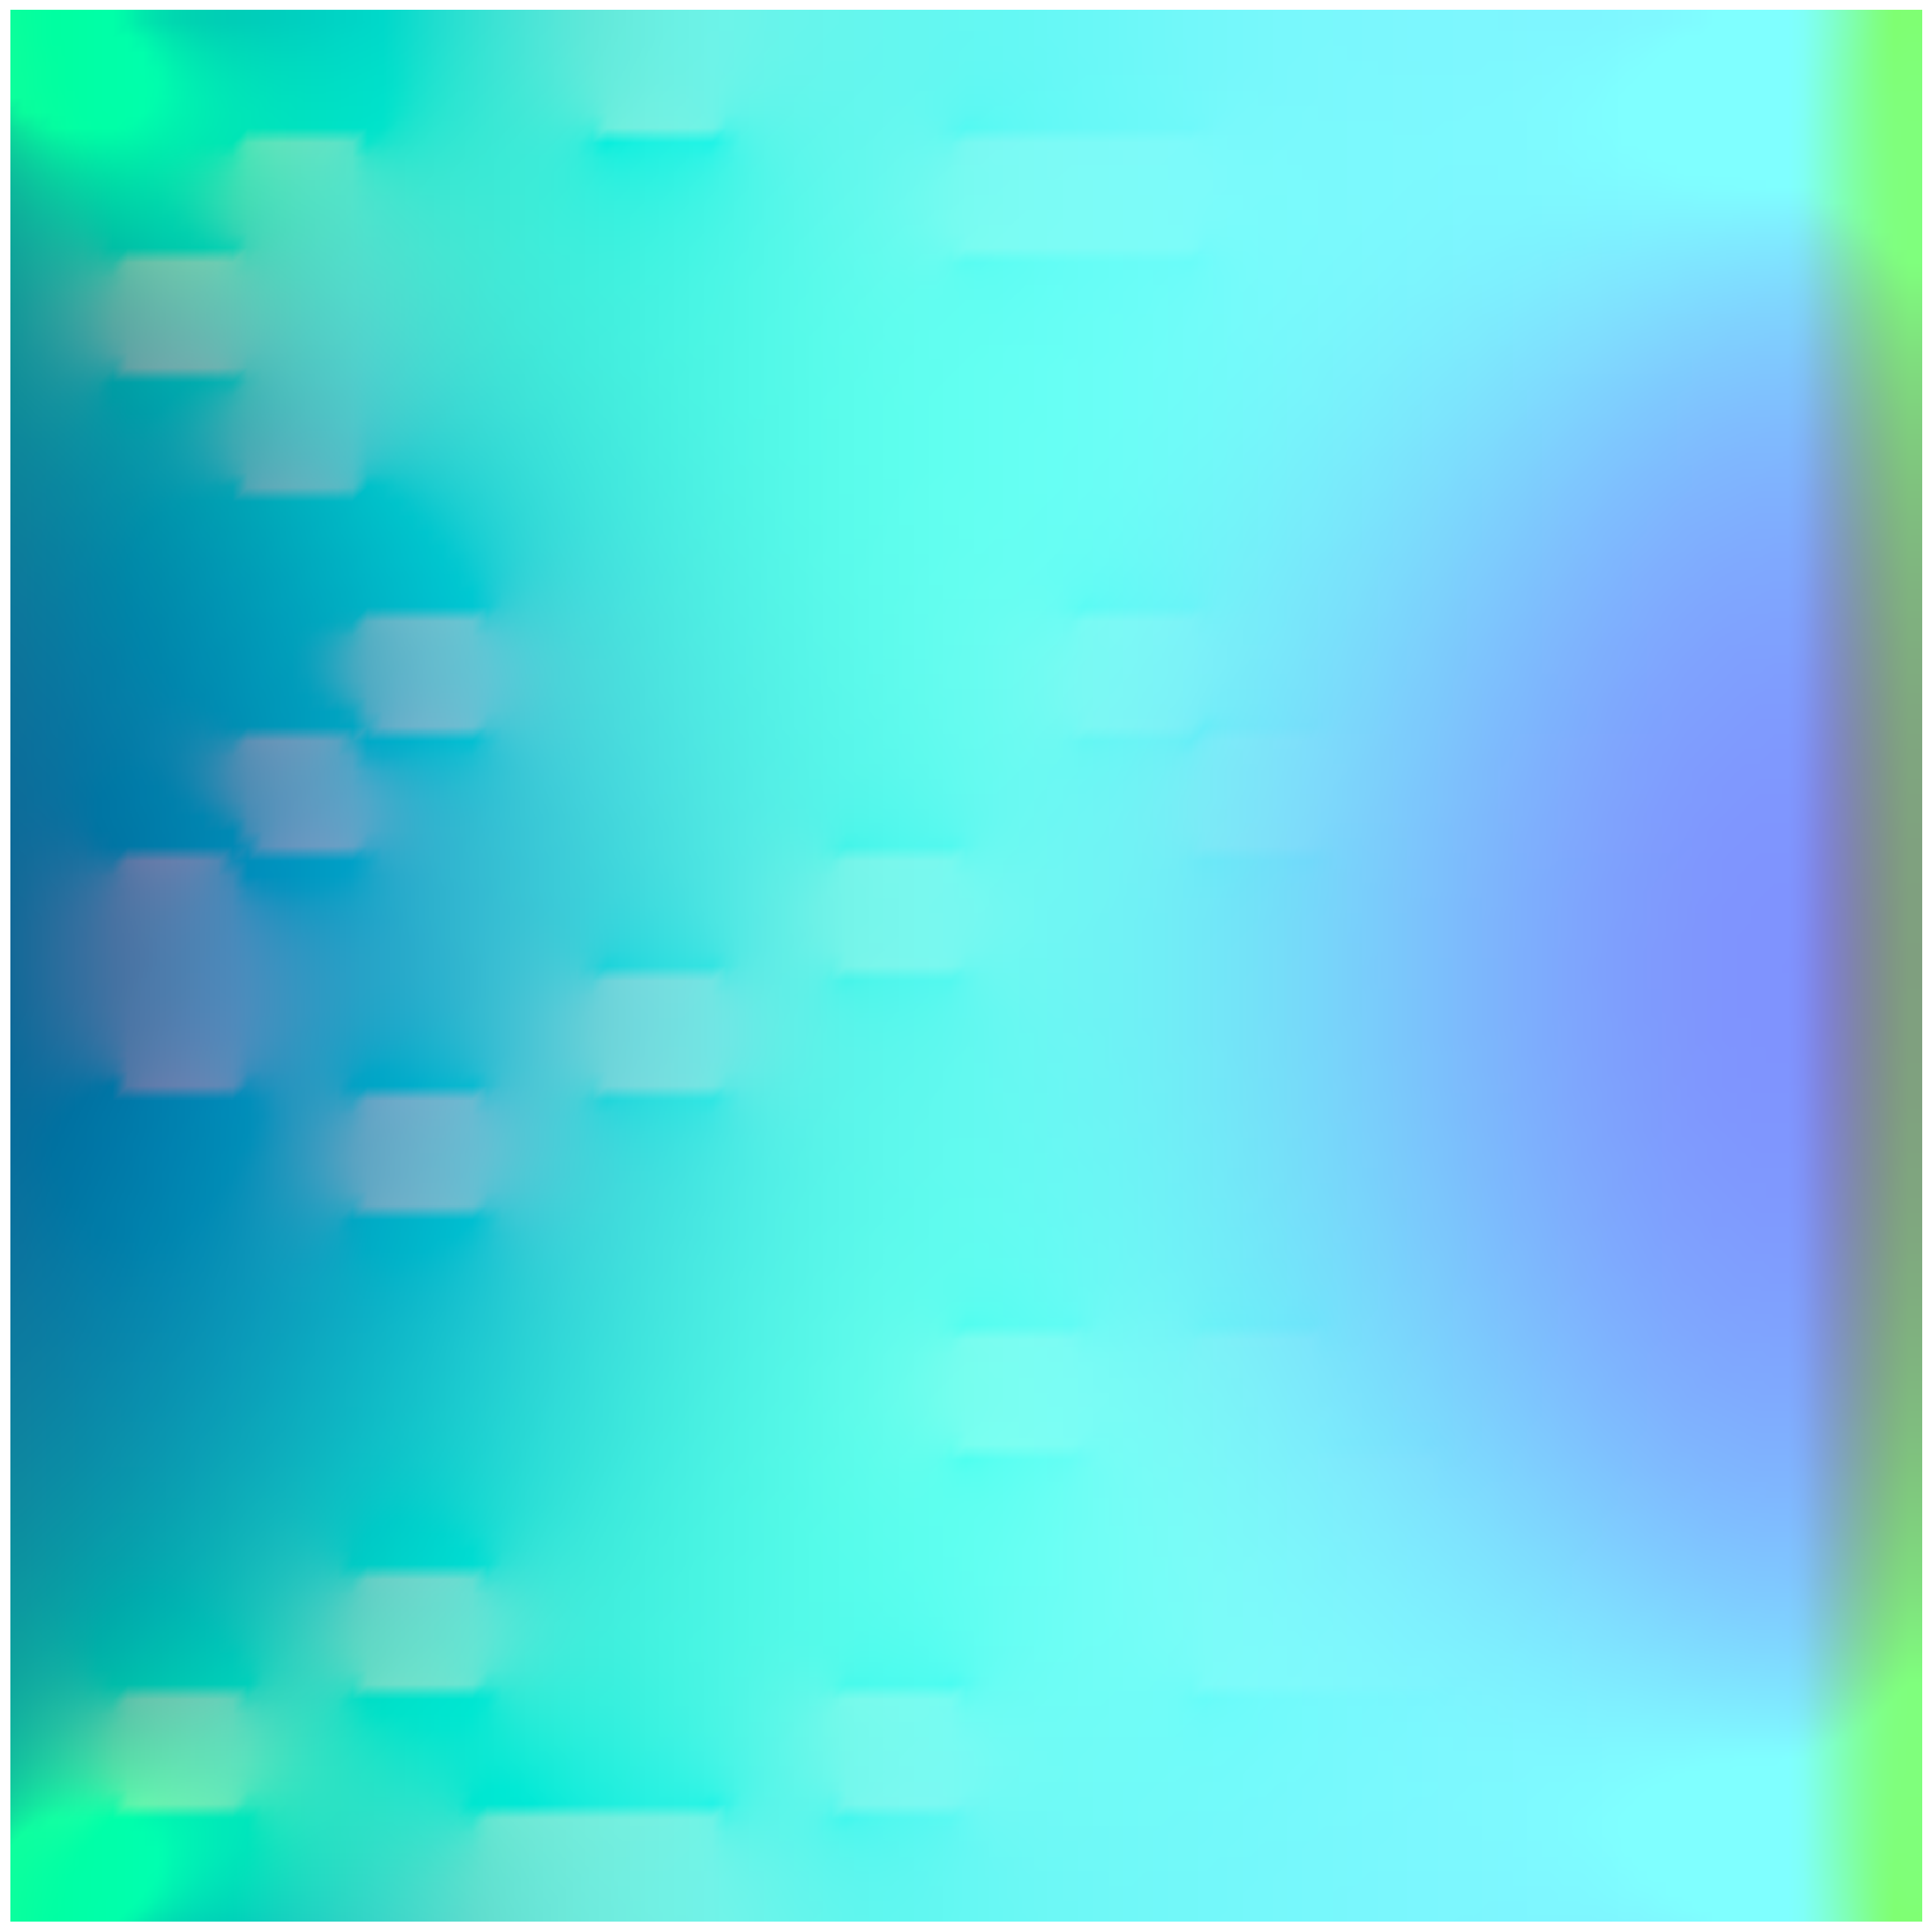
\includegraphics[width=0.5\linewidth]{figures/dummy}
  \caption{Do not state the obvious. Do not state the obvious. Do not state the obvious. Do not state the obvious. Do not state the obvious. Do not state the obvio.}
\end{figure}

Today data is often visualized as graphs to make it more readable and easier to understand and access. The problem with this is, that current research creates large datasets and the more data is visualized, the harder it gets to read the resulting graph. This predicament lead to the development of edge bundling techniques. These techniques allow graphs to become more readable and reveal patterns that were previously hidden. In this thesis I like to address certain issues with the current approaches and discuss possible solutions to them. 

One problem that is inherent in almost all current bundling techniques is the lack of a mathematical structure. Most methods just start bundling without a clue where the bundling should lead. For example the Force-Directed approach by Holten \cite{